\documentclass[onesided]{article}\usepackage[]{graphicx}\usepackage[]{color}
% maxwidth is the original width if it is less than linewidth
% otherwise use linewidth (to make sure the graphics do not exceed the margin)
\makeatletter
\def\maxwidth{ %
  \ifdim\Gin@nat@width>\linewidth
    \linewidth
  \else
    \Gin@nat@width
  \fi
}
\makeatother

\definecolor{fgcolor}{rgb}{0.345, 0.345, 0.345}
\newcommand{\hlnum}[1]{\textcolor[rgb]{0.686,0.059,0.569}{#1}}%
\newcommand{\hlstr}[1]{\textcolor[rgb]{0.192,0.494,0.8}{#1}}%
\newcommand{\hlcom}[1]{\textcolor[rgb]{0.678,0.584,0.686}{\textit{#1}}}%
\newcommand{\hlopt}[1]{\textcolor[rgb]{0,0,0}{#1}}%
\newcommand{\hlstd}[1]{\textcolor[rgb]{0.345,0.345,0.345}{#1}}%
\newcommand{\hlkwa}[1]{\textcolor[rgb]{0.161,0.373,0.58}{\textbf{#1}}}%
\newcommand{\hlkwb}[1]{\textcolor[rgb]{0.69,0.353,0.396}{#1}}%
\newcommand{\hlkwc}[1]{\textcolor[rgb]{0.333,0.667,0.333}{#1}}%
\newcommand{\hlkwd}[1]{\textcolor[rgb]{0.737,0.353,0.396}{\textbf{#1}}}%
\let\hlipl\hlkwb

\usepackage{framed}
\makeatletter
\newenvironment{kframe}{%
 \def\at@end@of@kframe{}%
 \ifinner\ifhmode%
  \def\at@end@of@kframe{\end{minipage}}%
  \begin{minipage}{\columnwidth}%
 \fi\fi%
 \def\FrameCommand##1{\hskip\@totalleftmargin \hskip-\fboxsep
 \colorbox{shadecolor}{##1}\hskip-\fboxsep
     % There is no \\@totalrightmargin, so:
     \hskip-\linewidth \hskip-\@totalleftmargin \hskip\columnwidth}%
 \MakeFramed {\advance\hsize-\width
   \@totalleftmargin\z@ \linewidth\hsize
   \@setminipage}}%
 {\par\unskip\endMakeFramed%
 \at@end@of@kframe}
\makeatother

\definecolor{shadecolor}{rgb}{.97, .97, .97}
\definecolor{messagecolor}{rgb}{0, 0, 0}
\definecolor{warningcolor}{rgb}{1, 0, 1}
\definecolor{errorcolor}{rgb}{1, 0, 0}
\newenvironment{knitrout}{}{} % an empty environment to be redefined in TeX

\usepackage{alltt}
\usepackage[T1]{fontenc}
\linespread{1.5} % Line spacing - Palatino needs more space between lines
\usepackage{microtype} % Slightly tweak font spacing for aesthetics

\usepackage[hmarginratio=1:1,columnsep=20pt]{geometry} % Document margins
%\usepackage{multicol} % Used for the two-column layout of the document
\usepackage[hang, small,labelfont=bf,up,textfont=it,up]{caption} % Custom captions under/above floats in tables or figures
\usepackage{booktabs} % Horizontal rules in tables
\usepackage{float} % Required for tables and figures in the multi-column environment - they need to be placed in specific locations with the [H] (e.g. \begin{table}[H])

\usepackage{lettrine} % The lettrine is the first enlarged letter at the beginning of the text
\usepackage{paralist} % Used for the compactitem environment which makes bullet points with less space between them

% to ignore texts: good for thank messages and paper submissions.
      % \fbox{\phantom{This text will be invisible too, but a box will be printed arround it.}}

\usepackage{abstract} % Allows abstract customization
\renewcommand{\abstractnamefont}{\normalfont\bfseries} % Set the "Abstract" text to bold
%\renewcommand{\abstracttextfont}{\normalfont\small\itshape} % Set the abstract itself to small italic text

\usepackage[]{titlesec} % Allows customization of titles
\renewcommand\thesection{\Roman{section}} % Roman numerals for the sections
\renewcommand\thesubsection{\Roman{subsection}} % Roman numerals for subsections
\titleformat{\section}[block]{\large\scshape\centering}{\thesection.}{1em}{} % Change the look of the section titles
\titleformat{\subsection}[block]{\large}{\thesubsection.}{1em}{} % Change the look of the section titles

\usepackage{fancybox, fancyvrb, calc}
\usepackage[svgnames]{xcolor}
\usepackage{physics}
\usepackage{epigraph}
\usepackage{longtable}
\usepackage{pdflscape}
\usepackage{graphics}
\usepackage{pbox} % \pbox{20cm}{This is the first \\ cell}
\usepackage{amsfonts}
\usepackage{amsmath}
\usepackage{amssymb}
\usepackage{rotating}
\usepackage{paracol}
\usepackage{textcomp}
\usepackage[export]{adjustbox}
\usepackage{afterpage}
\usepackage{filecontents}
\usepackage{color}
\usepackage{latexsym}
\usepackage{lscape}       %\begin{landscape} and \end{landscape}
\usepackage{wasysym}
\usepackage{dashrule}
\usepackage{marvosym} % face package
\usepackage{framed}
\usepackage{tree-dvips}
\usepackage{pgffor}
\usepackage[]{authblk}
\usepackage{setspace}
\usepackage{array}
\usepackage[latin1]{inputenc}
\usepackage{hyperref}     %desactivar para link rojos
\usepackage{graphicx}
\usepackage{dcolumn} % for R tables
\usepackage{multirow} % For multirow in tables
\usepackage{pifont}
\usepackage{listings}
\usepackage{bm}




% hypothesis / theorem package begin
\usepackage{amsthm}
\usepackage{thmtools}
\declaretheoremstyle[
spaceabove=6pt, spacebelow=6pt,
headfont=\normalfont\bfseries,
notefont=\mdseries, notebraces={(}{)},
bodyfont=\normalfont,
postheadspace=0.6em,
headpunct=:
]{mystyle}
\declaretheorem[style=mystyle, name=Hypothesis, preheadhook={\renewcommand{\thehyp}{H\textsubscript{\arabic{hyp}}}}]{hyp}

\usepackage{cleveref}
\crefname{hyp}{hypothesis}{hypotheses}
\Crefname{hyp}{Hypothesis}{Hypotheses}
% hypothesis / theorem package end


%----------------------------------------------------------------------------------------
% Other ADDS-ON
%----------------------------------------------------------------------------------------

% independence symbol \independent
\newcommand\independent{\protect\mathpalette{\protect\independenT}{\perp}}
\def\independenT#1#2{\mathrel{\rlap{$#1#2$}\mkern2mu{#1#2}}}







\hypersetup{
    bookmarks=true,         % show bookmarks bar?
    unicode=false,          % non-Latin characters in Acrobat's bookmarks
    pdftoolbar=true,        % show Acrobat's toolbar?
    pdfmenubar=true,        % show Acrobat's menu?
    pdffitwindow=true,     % window fit to page when opened
    pdfstartview={FitH},    % fits the width of the page to the window
    pdftitle={My title},    % title
    pdfauthor={Author},     % author
    pdfsubject={Subject},   % subject of the document
    pdfcreator={Creator},   % creator of the document
    pdfproducer={Producer}, % producer of the document
    pdfkeywords={keyword1} {key2} {key3}, % list of keywords
    pdfnewwindow=true,      % links in new window
    colorlinks=true,       % false: boxed links; true: colored links
    linkcolor=ForestGreen,          % color of internal links (change box color with linkbordercolor)
    citecolor=ForestGreen,        % color of links to bibliography
    filecolor=ForestGreen,      % color of file links
    urlcolor=ForestGreen           % color of external links
}

%\usepackage[nodayofweek,level]{datetime} % to have date within text

\newcommand{\LETT}[3][]{\lettrine[lines=4,loversize=.2,#1]{\smash{#2}}{#3}} % letrine customization



% comments on margin
  % Select what to do with todonotes: 
  % \usepackage[disable]{todonotes} % notes not showed
  \usepackage[draft]{todonotes}   % notes showed
  % usage: \todo{This is a note at margin}

\usepackage{cooltooltips}

%%% bib begin
\usepackage[american]{babel}
\usepackage{csquotes}
\usepackage[backend=biber,style=authoryear,dashed=false,doi=false,isbn=false,url=false,arxiv=false]{biblatex}
%\DeclareLanguageMapping{american}{american-apa}
\addbibresource{/Users/hectorbahamonde/Bibliografia_PoliSci/library.bib} 
\addbibresource{/Users/hectorbahamonde/Bibliografia_PoliSci/Bahamonde_BibTex2013.bib} 

% USAGES
%% use \textcite to cite normal
%% \parencite to cite in parentheses
%% \footcite to cite in footnote
%% the default can be modified in autocite=FOO, footnote, for ex. 
%%% bib end

\usepackage{fancyhdr} % Headers and footers
\pagestyle{fancy} % All pages have headers and footers
\fancyhead{} % Blank out the default header
\fancyfoot{} % Blank out the default footer
\fancyhead[C]{MLE para Outcomes Binarios: Diagn\'osticos} % Custom header text
\fancyfoot[RO,LE]{\thepage} % Custom footer text
\IfFileExists{upquote.sty}{\usepackage{upquote}}{}
\begin{document}
% DOCUMENT ID
%----------------------------------------------------------------------------------------
% CONTENT
%----------------------------------------------------------------------------------------

%\graphicspath{
%{/Users/hectorbahamonde/RU/Term5/Experiments_Redlawsk/Experiment/Data/}
%}



%%%%%%%%%%%%%%%%%%%%%%%%%%%%%%%%%%%%%%%%%%%%%%
% begin knitr stuff


%%%%%%%%%%%%%%%%%%%%%%%%%%%%%%%%%%%%%%%%%%%%%%





\hspace{-5mm}{\bf Profesor}: H\'ector Bahamonde, PhD.\\
\texttt{e:}\href{mailto:hector.bahamonde@uoh.cl}{\texttt{hector.bahamonde@uoh.cl}}\\
\texttt{w:}\href{http://www.hectorbahamonde.com}{\texttt{www.hectorbahamonde.com}}\\
{\bf Curso}: MLE.\\
\hspace{-5mm}{\bf TA}: Gonzalo Barr\'ia.

\section{Diagn\'osticos}

Al igual que en el ``mundo'' OLS, existen formas para evaluar cu\'an bueno (o malo) es nuestro modelo. {\color{red}Qu\'e tipo de diagn\'osticos existen en el ``mundo'' OLS?}

Recuerda que en OLS, el residuo $\epsilon_{i}$ es la diferencia entre lo que predecimos y lo que observamos, o $\epsilon_{i}=y_{i}-x_{ij}\beta_{j}$ (donde $y_{i}$ son los valores de la variable dependiente para observaci\'on $i$, $x_{ij}$ son los $j$ variables dependientes para cada una de las observaciones $i$, y $\beta_{j}$ son los $j$ par\'ametros estimados). 

Si recuerdas bien, $E(\epsilon_{i})=0$ y homoesqued\'astico (varianza constante). En MLE, es bastante similar, ``pero ni tanto'':

\begin{itemize}
\item En vez de un $\beta_{j}$ que se multiplica por cada $x_{ij}$, hablamos de la probabilidad $\pi_{i}$ de que observemos la realizaci\'on del evento en el sujeto $i$. O m\'as formalmente, $\pi_{i}=E(y_{i}|{\mathbf x}_{i}) = Pr(y_{i}=1|{\mathbf x}_{i})$. Nota que ${\mathbf x}_{i}$ es una matriz ({\color{red}por qu\'e?}). 
\item Ademas, si quisieras comparar diagn\'osticos entre distintos modelos y con distintas bases de datos, {\bf no puedes}. Esto es una limitante de MLE: al estar diagnosticando modelos (con las herramientas que veremos hoy), {\bf s\'olo podr\'as hacerlo entre modelos que se hayan estimado con la \emph{misma} base de datos}.
\end{itemize}


\section{An\'alisis de Residuos}

El primer enfoque para diagnosticar un modelo GLM es mirando sus residuos.

\paragraph{Residuos Pearson} Debido a que $y_{i}$ es una variable bimodal, la distribuci\'on de $Pr(y_{i}=1|{\mathbf x}_{i})$ es sigmoidal. En consecuencia, las desviaciones $y_{i}-\pi_{i}$ son heteroesqued\'asticos (no constantes). Por estas razones, en MLE no trabajamos con residuos del tipo $e_{i} = y_{i} - \hat y_{i} $, sino que con un tipo de residuos estandarizados llamados ``Residuos Pearson'' $r_{i}$:

\begin{equation}\label{r:pearson}
r_{i} = \frac{y_{i}-\hat \pi_{i}}{\sqrt{\hat \pi_{i}(1-\hat \pi_{i})}}
\end{equation}

donde $\sqrt{\hat \pi_{i}(1-\hat \pi_{i})}$ es la varianza. Cuando $r_{i}$ es grande, eso indica que existe un mal ``fit'' (o ``ajuste'', i.e. nuestra l\'inea de regresi\'on pasa lejos de las observaciones. Si te fijas, cada observaci\'on $i$ tiene su contribuci\'on al error total del modelo: hay un $r_{i}$ para cada observaci\'on $i$. Veamos ahora un ``\emph{index plot}'' donde graficamos todos los $r_{i}$ de manera ordenada (o ``por \'indice'': el primer $r_{1}$, despues el segundo $r_{2}$, etc.). 

Carguemos los datos.


\begin{knitrout}
\definecolor{shadecolor}{rgb}{0.969, 0.969, 0.969}\color{fgcolor}\begin{kframe}
\begin{alltt}
\hlstd{dat} \hlkwb{<-} \hlkwd{read.csv}\hlstd{(}\hlstr{"https://stats.idre.ucla.edu/stat/data/binary.csv"}\hlstd{)}
\hlkwd{head}\hlstd{(dat)}
\end{alltt}
\begin{verbatim}
##   admit gre  gpa rank
## 1     0 380 3.61    3
## 2     1 660 3.67    3
## 3     1 800 4.00    1
## 4     1 640 3.19    4
## 5     0 520 2.93    4
## 6     1 760 3.00    2
\end{verbatim}
\begin{alltt}
\hlkwd{summary}\hlstd{(dat)}
\end{alltt}
\begin{verbatim}
##      admit             gre             gpa             rank      
##  Min.   :0.0000   Min.   :220.0   Min.   :2.260   Min.   :1.000  
##  1st Qu.:0.0000   1st Qu.:520.0   1st Qu.:3.130   1st Qu.:2.000  
##  Median :0.0000   Median :580.0   Median :3.395   Median :2.000  
##  Mean   :0.3175   Mean   :587.7   Mean   :3.390   Mean   :2.485  
##  3rd Qu.:1.0000   3rd Qu.:660.0   3rd Qu.:3.670   3rd Qu.:3.000  
##  Max.   :1.0000   Max.   :800.0   Max.   :4.000   Max.   :4.000
\end{verbatim}
\end{kframe}
\end{knitrout}

Ahora estimemos el modelo:

\begin{knitrout}
\definecolor{shadecolor}{rgb}{0.969, 0.969, 0.969}\color{fgcolor}\begin{kframe}
\begin{alltt}
\hlstd{logit.1} \hlkwb{<-} \hlkwd{glm}\hlstd{(admit} \hlopt{~} \hlstd{gre} \hlopt{+} \hlstd{gpa,} \hlkwc{data} \hlstd{= dat,} \hlkwc{family} \hlstd{=} \hlkwd{binomial}\hlstd{(}\hlkwc{link} \hlstd{=} \hlstr{"logit"}\hlstd{))}
\hlkwd{summary}\hlstd{(logit.1)}
\end{alltt}
\begin{verbatim}
## 
## Call:
## glm(formula = admit ~ gre + gpa, family = binomial(link = "logit"), 
##     data = dat)
## 
## Deviance Residuals: 
##     Min       1Q   Median       3Q      Max  
## -1.2730  -0.8988  -0.7206   1.3013   2.0620  
## 
## Coefficients:
##              Estimate Std. Error z value   Pr(>|z|)    
## (Intercept) -4.949378   1.075093  -4.604 0.00000415 ***
## gre          0.002691   0.001057   2.544     0.0109 *  
## gpa          0.754687   0.319586   2.361     0.0182 *  
## ---
## Signif. codes:  0 '***' 0.001 '**' 0.01 '*' 0.05 '.' 0.1 ' ' 1
## 
## (Dispersion parameter for binomial family taken to be 1)
## 
##     Null deviance: 499.98  on 399  degrees of freedom
## Residual deviance: 480.34  on 397  degrees of freedom
## AIC: 486.34
## 
## Number of Fisher Scoring iterations: 4
\end{verbatim}
\end{kframe}
\end{knitrout}

Y usando la funci\'on \texttt{rstandard} calcularemos $r_{i}$

\begin{knitrout}
\definecolor{shadecolor}{rgb}{0.969, 0.969, 0.969}\color{fgcolor}\begin{kframe}
\begin{alltt}
\hlstd{r} \hlkwb{=} \hlkwd{rstandard}\hlstd{(logit.1)}
\hlkwd{head}\hlstd{(r)}
\end{alltt}
\begin{verbatim}
##          1          2          3          4          5          6 
## -0.7300511  1.3559165  1.0930693  1.5430303 -0.6844243  1.4711335
\end{verbatim}
\end{kframe}
\end{knitrout}

Como ves, cada observaci\'on $i$ tiene su propio error (la distancia dada por $y_{i}-\hat \pi_{i}$). 

Hagamos el ``index plot'':

\begin{knitrout}
\definecolor{shadecolor}{rgb}{0.969, 0.969, 0.969}\color{fgcolor}\begin{kframe}
\begin{alltt}
\hlkwd{plot}\hlstd{(}\hlnum{1}\hlopt{:}\hlkwd{nrow}\hlstd{(dat),} \hlcom{# Numero de Obs}
     \hlstd{r,} \hlcom{# y}
     \hlkwc{ylab}\hlstd{=}\hlstr{"Residuos Estandarizados"}\hlstd{,}
     \hlkwc{xlab}\hlstd{=}\hlstr{"Index (Numero de Obs)"}\hlstd{)}
\hlkwd{abline}\hlstd{(}\hlnum{0}\hlstd{,} \hlnum{0}\hlstd{)}
\hlkwd{abline}\hlstd{(}\hlnum{2}\hlstd{,} \hlnum{0}\hlstd{)}
\hlkwd{abline}\hlstd{(}\hlopt{-}\hlnum{2}\hlstd{,} \hlnum{0}\hlstd{)}
\end{alltt}
\end{kframe}

{\centering 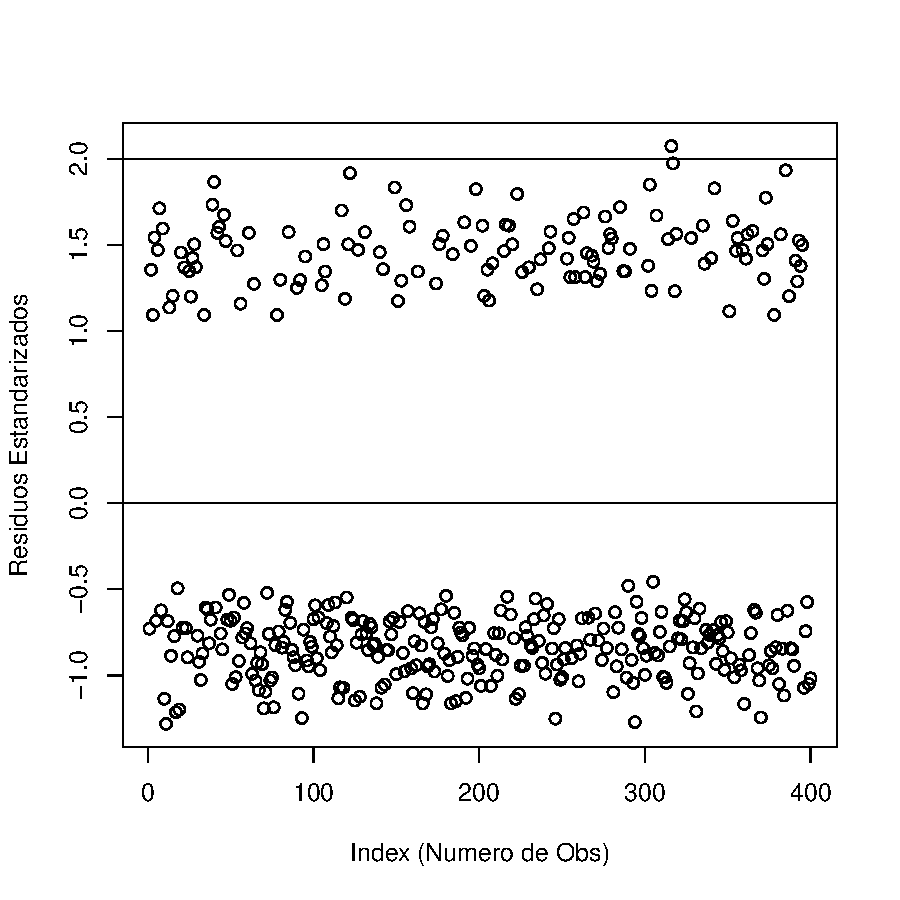
\includegraphics[width=\maxwidth]{figure/rindexplot-1} 

}



\end{knitrout}

En la figura vemos que hay un \emph{outlier} (fuera de las dos desviaciones est\'andar). 

Veamos ahora c\'omo se ven los residuos Pearson $r_{i}$:

\begin{knitrout}
\definecolor{shadecolor}{rgb}{0.969, 0.969, 0.969}\color{fgcolor}\begin{kframe}
\begin{alltt}
\hlkwd{plot}\hlstd{(}\hlkwd{density}\hlstd{(}\hlkwd{rstandard}\hlstd{(logit.1,} \hlkwc{type}\hlstd{=}\hlstr{'pearson'}\hlstd{)))}
\end{alltt}
\end{kframe}

{\centering 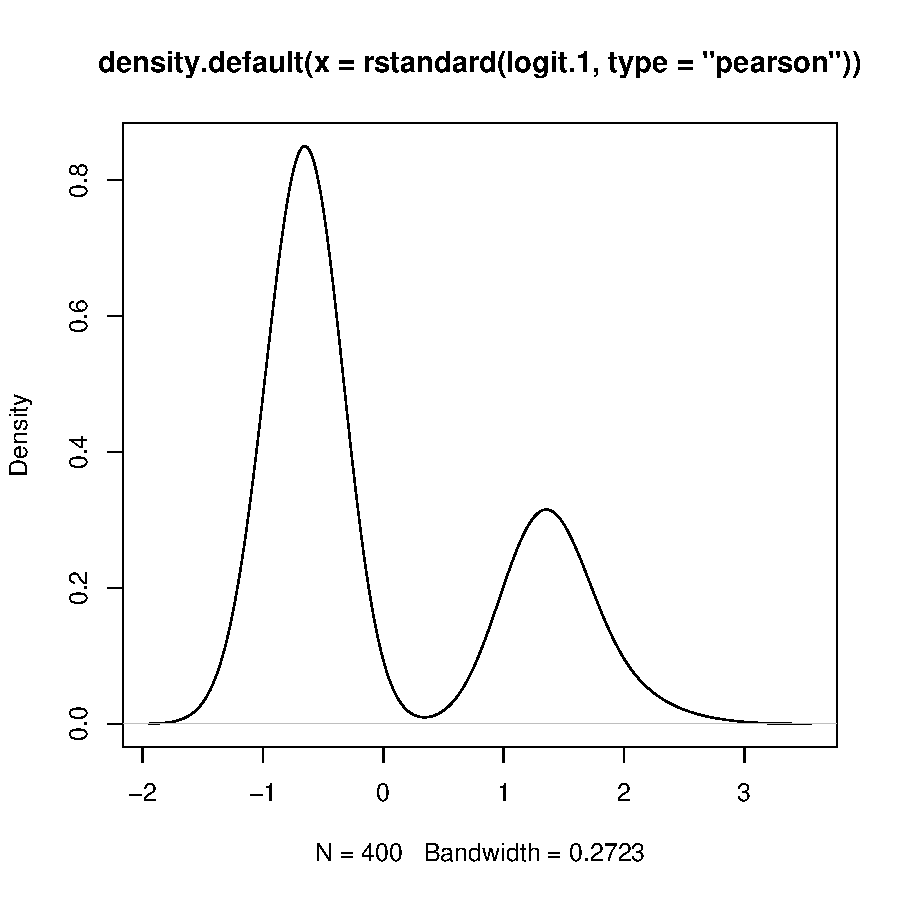
\includegraphics[width=\maxwidth]{figure/r:pearson:plot-1} 

}



\end{knitrout}


\begin{knitrout}
\definecolor{shadecolor}{rgb}{0.969, 0.969, 0.969}\color{fgcolor}\begin{kframe}
\begin{alltt}
\hlkwd{p_load}\hlstd{(car)}
\hlkwd{residualPlots}\hlstd{(logit.1,} \hlkwc{layout}\hlstd{=}\hlkwd{c}\hlstd{(}\hlnum{3}\hlstd{,}\hlnum{1}\hlstd{))}
\end{alltt}
\end{kframe}

{\centering 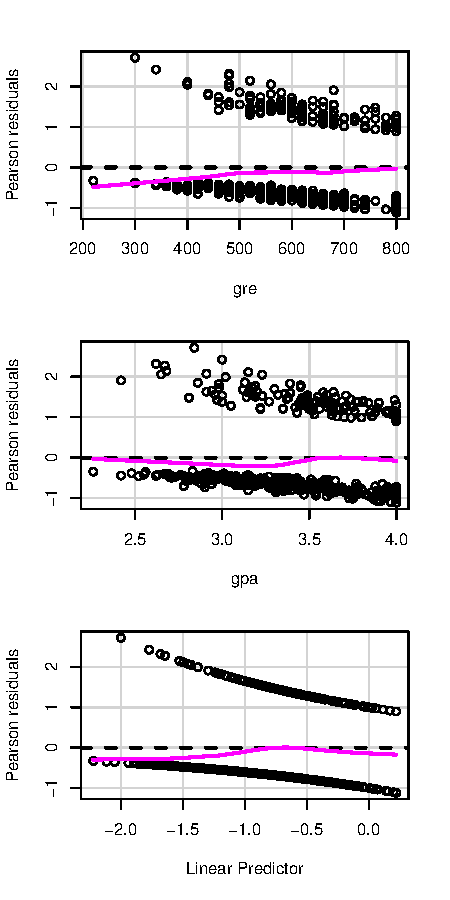
\includegraphics[width=\maxwidth]{figure/residual:plot-1} 

}


\begin{kframe}\begin{verbatim}
##     Test stat Pr(>|Test stat|)
## gre    0.1197           0.7293
## gpa    0.1613           0.6880
\end{verbatim}
\end{kframe}
\end{knitrout}

\paragraph{Cook's Distance} Una de las ventajas del an\'alisis de residuos en GLM via MLE, es que podemos extraer casi todo lo que hemos aprendido en OLS. Podemos aproximar el \emph{Cook's Distance} ($D_{i}$) para GLMs de la siguiente manera:

\begin{equation}
D_{i} = (\frac{r_{i}}{1-\cal{H}})^{2} \times \frac{\cal{H}}{\sigma \times K}
\end{equation}

donde $r_{i}$ est\'a definido en \autoref{r:pearson}, $\cal{H}$ es una ``hat matrix'' (funci\'on que mapea $y_{i} \rightarrow \hat{y}_{i}$), $K$ el n\'umero de par\'ametros, y $\sigma$ es la dispersi\'on del modelo (varianza). En los modelos log\'isticos y Poisson $\sigma=1$.


Grafiquemos $D_{i}$:

\begin{knitrout}
\definecolor{shadecolor}{rgb}{0.969, 0.969, 0.969}\color{fgcolor}\begin{kframe}
\begin{alltt}
\hlkwd{p_load}\hlstd{(car)}
\hlkwd{influenceIndexPlot}\hlstd{(logit.1,} \hlkwc{vars}\hlstd{=}\hlkwd{c}\hlstd{(}\hlstr{"Cook"}\hlstd{))}
\end{alltt}
\end{kframe}

{\centering 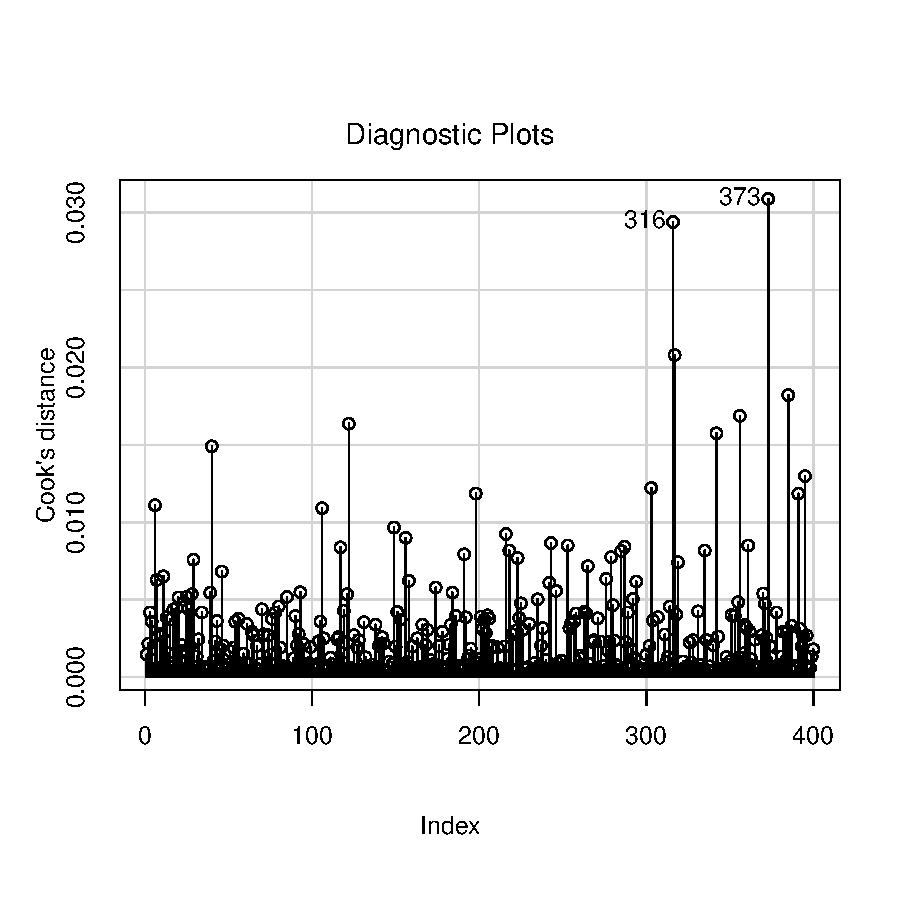
\includegraphics[width=\maxwidth]{figure/d:plot-1} 

}



\end{knitrout}


\paragraph{DFFIT} Otra manera de pensar la influencia que tiene cada observaci\'on es haciendo una regresi\'on secuencial en la que vamos sacando esa observaci\'on, una a la vez. Define \emph{DFFIT} como,  

\begin{equation}\label{DFFIT}
DFFIT_{i} = \hat{y}_{i} - \hat{y_{i}}_{(i)}
\end{equation}

donde \emph{DFFIT} es el cambio en el valor predicho para la observaci\'on $i$ (o ``\emph{fit}'') cuando $i$ es dejada afuera de la regresi\'on. La versi\'on m\'as usada del \emph{DFFIT} es la versi\'on estandarizada (es decir, que podemos usar para comparar) llamada \emph{DFFITS} (con una ``s'' al final de ``standarized''). La \'unica diferencia es que \'esta est\'a dividida por por el error est\'andar que aporta la observaci\'on $SE_{i}$ (y multiplicado por la ra\'iz cuadrada del ``\emph{leverage}'' o influencia de la observaci\'on $i$), $\sqrt{h_{i}}$\footnote{El ``leverage'' de $i$ est\'a dado por: \begin{equation}x(x^{T}x)-1x^{T}\end{equation}}. En otras palabras,


\begin{equation}\label{DFFIT}
DFFITS_{i} = \frac{DFFIT}{SE_{i}\sqrt{h_{i}}}
\end{equation}

Calculemos el vector de DFFITS, y veamos los primeros diez valores.

\begin{knitrout}
\definecolor{shadecolor}{rgb}{0.969, 0.969, 0.969}\color{fgcolor}\begin{kframe}
\begin{alltt}
\hlstd{dffits} \hlkwb{=} \hlkwd{dffits}\hlstd{(logit.1)} \hlcom{# calcula el vector de dffits}
\hlkwd{as.numeric}\hlstd{(dffits)[}\hlnum{1}\hlopt{:}\hlnum{10}\hlstd{]} \hlcom{# ve los primeros 10.}
\end{alltt}
\begin{verbatim}
##  [1] -0.07958515  0.08100147  0.12336778  0.09660158 -0.04878515  0.17588014
##  [7]  0.11753107 -0.05089782  0.08350179 -0.09699958
\end{verbatim}
\end{kframe}
\end{knitrout}

Los \emph{DFFITS} tienen valores cr\'iticos (\emph{critical values}, o ``cv''). Si la observaci\'on supera ese valor cr\'itico, es considerada ``\emph{influential}''. Los valores cr\'iticos est\'an dados por el siguiente c\'alculo,

\begin{equation}\label{DFFIT.cv} 
\text{cv}_{\text{DFFITS}} = 2 \times \sqrt{\frac{k}{n}}
\end{equation}

donde $k$ es el n\'umero de param\'etros, y $n$ el n\'umero de observaciones. Calculemos $\text{cv}_{\text{DFFITS}}$ en \texttt{R}:

\begin{knitrout}
\definecolor{shadecolor}{rgb}{0.969, 0.969, 0.969}\color{fgcolor}\begin{kframe}
\begin{alltt}
\hlstd{n} \hlkwb{=} \hlkwd{nrow}\hlstd{(dat)}
\hlstd{k} \hlkwb{=} \hlkwd{length}\hlstd{(logit.1}\hlopt{$}\hlstd{coefficients)}\hlopt{-}\hlnum{1}
\hlstd{cv} \hlkwb{=} \hlnum{2}\hlopt{*}\hlkwd{sqrt}\hlstd{(k}\hlopt{/}\hlstd{n)}
\end{alltt}
\end{kframe}
\end{knitrout}

Ahora grafiquemos la influencia de cada $i$, pero siempre tomando en cuenta los $\text{cv}_{\text{DFFITS}}$.


\begin{knitrout}
\definecolor{shadecolor}{rgb}{0.969, 0.969, 0.969}\color{fgcolor}\begin{kframe}
\begin{alltt}
\hlkwd{plot}\hlstd{(}\hlkwd{dffits}\hlstd{(logit.1))} \hlcom{# grafico de dffits}
\hlkwd{abline}\hlstd{(}\hlkwc{h} \hlstd{= cv,} \hlkwc{lty} \hlstd{=} \hlnum{2}\hlstd{)} \hlcom{# anadir cv hacia arriba}
\hlkwd{abline}\hlstd{(}\hlkwc{h} \hlstd{=} \hlopt{-}\hlstd{cv,} \hlkwc{lty} \hlstd{=} \hlnum{2}\hlstd{)} \hlcom{# anadir cv hacia abajo}
\end{alltt}
\end{kframe}

{\centering 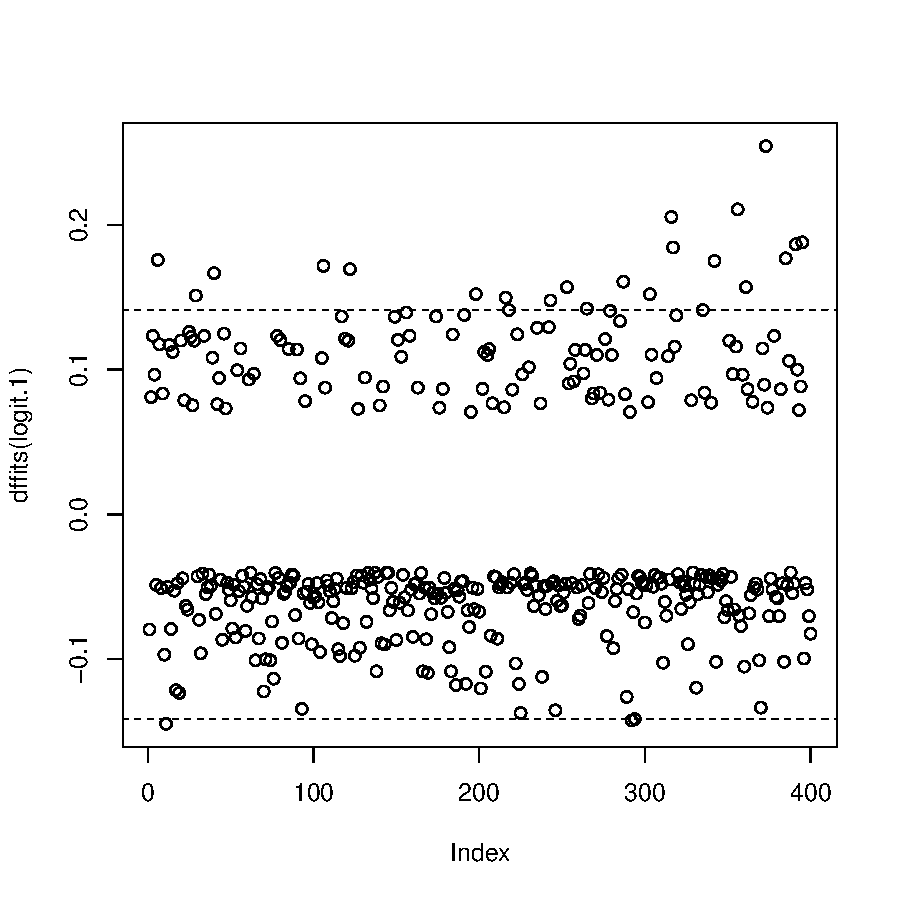
\includegraphics[width=\maxwidth]{figure/DFFITS:p-1} 

}



\end{knitrout}

Como puedes ver existen varias observacioens ``influyentes''. Vayamos a \texttt{R} y tratemos de identificar cuales son esas observaciones influyentes usando la siguiente l\'inea:

\begin{verbatim}
identify(row.names(dat), dffits(logit.1), row.names(dat), plot=TRUE)
\end{verbatim}

\paragraph{DFBETA} Una manera hom\'ologa es ver cu\'anto cambian los par\'ametros estimados $\hat\beta_{k}$ al excluir cada $i$ a la vez. Estos son los $DFBETA$ y est\'an dados por el siguiente c\'alculo,

\begin{equation}\label{DFBETA}
DFBETA_{i} = \bm{\beta}-\bm{\beta}_{(-i)}
\end{equation}

Donde $\bm{\beta}$ son todos los par\'ametros estimados y $\bm{\beta}_{(-i)}$ son todos los par\'ametros estimados quitando la observaci\'on $i$.

De manera analoga, existe un correlato estandarizado \emph{DFBETAS} dado por, 

\begin{equation}\label{DFBETA}
DFBETAS_{i} = \frac{DFBETA}{\sqrt{\hat{\sigma^{2}}_{i}(x^{T}x)^{-1}}}
\end{equation}

Esta estandarizaci\'on nos permite establecer un par\'ametro de comparaci\'on: toda observaci\'on $i$ que tenga un $DFBETAS_{i}$ mayor a 1 es considerada ``sospechosa'' de tener influencia.

Extraigamos los $DFBETAS_{i}$ para cada uno de los $k$ parametros (en nuestro caso, 3). Por simplicidad veamos los primeros.

\begin{knitrout}
\definecolor{shadecolor}{rgb}{0.969, 0.969, 0.969}\color{fgcolor}\begin{kframe}
\begin{alltt}
\hlstd{dfbetas} \hlkwb{=} \hlkwd{dfbetas}\hlstd{(logit.1)}
\hlkwd{head}\hlstd{(dfbetas)}
\end{alltt}
\begin{verbatim}
##    (Intercept)         gre         gpa
## 1 -0.007503563 0.071946453 -0.03756627
## 2 -0.037877366 0.020634219  0.03167665
## 3 -0.092543108 0.072844646  0.05354764
## 4  0.044668602 0.042084994 -0.06093219
## 5 -0.042668687 0.008568481  0.03391040
## 6  0.056065572 0.136316436 -0.12687735
\end{verbatim}
\end{kframe}
\end{knitrout}

Ahora usemos la funci\'on \texttt{dfbetaPlots} para graficar con un s\'olo comando los dos graficos que necesitamos (\texttt{gre} y \texttt{gpa}),

\begin{knitrout}
\definecolor{shadecolor}{rgb}{0.969, 0.969, 0.969}\color{fgcolor}\begin{kframe}
\begin{alltt}
\hlkwd{p_load}\hlstd{(car)}
\hlkwd{dfbetaPlots}\hlstd{(logit.1)}
\end{alltt}
\end{kframe}

{\centering 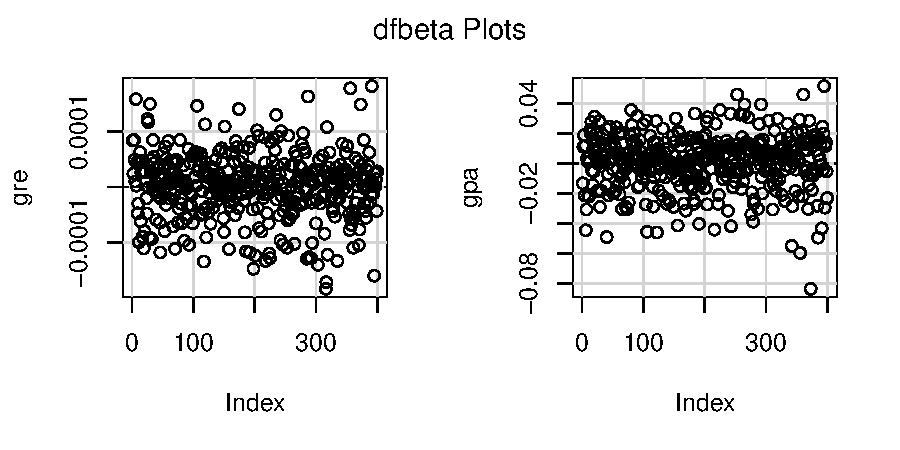
\includegraphics[width=\maxwidth]{figure/DFBETAS:p-1} 

}



\end{knitrout}

En este caso no vemos grandes alejamientos del par\'ametro.

\section{Goodness of Fit}

Otra de las preguntas que siempre debemos hacer es cu\'an bien (o mal) nuestro modelo ($\bm{x}_{i}\bm{\beta}_{K}$) se ajusta a la variable dependiente $y_{i}$. Esto se llama \emph{goodness of fit}.

\paragraph{pseudo-$r^{2}$} El primer indicador de ajuste es el pseudo$-r^{2}$. En MLE los coeficientes no est\'an dise\~nados para minimizar varianza (sino que para maximizar (log)likelihood). Entonces, el enfoque clasico del $r^{2}$ no nos sirve aqu\'i. Adem\'as, recuerda que si bien el $r^2$ pod\'ia ser comparado entre modelos estimados con distintas bases de datos, en MLE el pseudo-$r^{2}$ {\bf s\'olo puede ser comparado con modelos estimados con la misma base de datos} (esto es porque en MLE todo es relativo no absoluto). Recuerda: el $r^{2}$ en OLS significa ``el porcentaje de varianza explicada''---pero ve \textcite{King1986}. Y el $r^{2}$ pod\'ia (en OLS) ser comparado entre distintos modelos estimados con distintas bases de datos.

En el mundo MLE existen varios indicadores que se asemejan al $r^{2}$, por eso ellos son ``pseudo'' $r^{2}$. El m\'as utilizado es el de McFadden dado por,

\begin{equation}\label{McFadden}
r^{2}_{\text{McFadden}} = 1 - \frac{log(L)}{log(L_{null})}
\end{equation}

De manera an\'aloga, es un radio que varia entre 0 y 1. Pero su significado no est\'a dado en t\'erminos de ``varianza explicada''. Si te fijas, es el radio entre el log-likelihood del modelo entero (``\emph{unrestricted}'') comparado modelo con s\'olo el intercepto---``\emph{restricted}'', es decir, cuando todos los $x$ del modelo son 0). 

Para calcular el $L_{null}$, estimemos el modelo,

\begin{knitrout}
\definecolor{shadecolor}{rgb}{0.969, 0.969, 0.969}\color{fgcolor}\begin{kframe}
\begin{alltt}
\hlstd{logit.null} \hlkwb{<-} \hlkwd{glm}\hlstd{(admit} \hlopt{~} \hlnum{1}\hlstd{,} \hlkwc{data} \hlstd{= dat,} \hlkwc{family} \hlstd{=} \hlkwd{binomial}\hlstd{(}\hlkwc{link} \hlstd{=} \hlstr{"logit"}\hlstd{))}
\hlkwd{summary}\hlstd{(logit.null)}
\end{alltt}
\begin{verbatim}
## 
## Call:
## glm(formula = admit ~ 1, family = binomial(link = "logit"), data = dat)
## 
## Deviance Residuals: 
##     Min       1Q   Median       3Q      Max  
## -0.8741  -0.8741  -0.8741   1.5148   1.5148  
## 
## Coefficients:
##             Estimate Std. Error z value         Pr(>|z|)    
## (Intercept)  -0.7653     0.1074  -7.125 0.00000000000104 ***
## ---
## Signif. codes:  0 '***' 0.001 '**' 0.01 '*' 0.05 '.' 0.1 ' ' 1
## 
## (Dispersion parameter for binomial family taken to be 1)
## 
##     Null deviance: 499.98  on 399  degrees of freedom
## Residual deviance: 499.98  on 399  degrees of freedom
## AIC: 501.98
## 
## Number of Fisher Scoring iterations: 4
\end{verbatim}
\end{kframe}
\end{knitrout}

Ahora, capturemos ambos log-likelihoods,

\begin{knitrout}
\definecolor{shadecolor}{rgb}{0.969, 0.969, 0.969}\color{fgcolor}\begin{kframe}
\begin{alltt}
\hlkwd{logLik}\hlstd{(logit.1)}
\end{alltt}
\begin{verbatim}
## 'log Lik.' -240.172 (df=3)
\end{verbatim}
\begin{alltt}
\hlkwd{logLik}\hlstd{(logit.null)}
\end{alltt}
\begin{verbatim}
## 'log Lik.' -249.9883 (df=1)
\end{verbatim}
\end{kframe}
\end{knitrout}

y computemos $r^{2}_{\text{McFadden}}$,

\begin{knitrout}
\definecolor{shadecolor}{rgb}{0.969, 0.969, 0.969}\color{fgcolor}\begin{kframe}
\begin{alltt}
\hlnum{1}\hlopt{-}\hlstd{(}\hlkwd{logLik}\hlstd{(logit.1)}\hlopt{/}\hlkwd{logLik}\hlstd{(logit.null))}
\end{alltt}
\begin{verbatim}
## 'log Lik.' 0.03926692 (df=3)
\end{verbatim}
\end{kframe}
\end{knitrout}

En este caso vemos que el $log(L)$ (modelo con par\'ametros) no alcanza a superar por tanto m\'as al $log(L_{null})$ (modelo sin par\'ametros). El $r^{2}_{\text{McFadden}}$ es casi 10\%. 

Aunque este indicador es intiutivo, conceptualmente es deficiente: {\bf el modelo que explica toda la varianza existente es un modelo que tiene todas las variables posibles de existir}. 


\paragraph{Information Criteria} Existen mejores maneras de referirse al ajuste del modelo (``\emph{goodness of fit}''). Hay dos tipos b\'asicos de criterios de informaci\'on. 

\begin{enumerate}
  \item BIC: Bayesian Information Criteria, dado por $k\times ln(n)-2ln(\hat{l})$.
  \item AIC: Akaike Information Criteria, dado por $2k-2ln(\hat{l})$.
\end{enumerate}

donde $k$ es el n\'umero de par\'ametros, $n$ el n\'umero de observaciones, y $\hat{l}$ el likelihood estimado. Nota que ambos son muy parecidos. {\bf En ambos criterios, el n\'umero m\'as peque\~no sugiere un mejor modelo}. 

Ahora comparemos el BIC para el \texttt{logit.1} y el \texttt{logit.null} (ambos estimados usando la misma base de datos). 

\begin{knitrout}
\definecolor{shadecolor}{rgb}{0.969, 0.969, 0.969}\color{fgcolor}\begin{kframe}
\begin{alltt}
\hlkwd{BIC}\hlstd{(logit.1,logit.null)}
\end{alltt}
\begin{verbatim}
##            df      BIC
## logit.1     3 498.3184
## logit.null  1 505.9680
\end{verbatim}
\end{kframe}
\end{knitrout}

Ahora comparemos el AIC para el \texttt{logit.1} y el \texttt{logit.null} (ambos estimados usando la misma base de datos). 

\begin{knitrout}
\definecolor{shadecolor}{rgb}{0.969, 0.969, 0.969}\color{fgcolor}\begin{kframe}
\begin{alltt}
\hlkwd{AIC}\hlstd{(logit.1,logit.null)}
\end{alltt}
\begin{verbatim}
##            df      AIC
## logit.1     3 486.3440
## logit.null  1 501.9765
\end{verbatim}
\end{kframe}
\end{knitrout}


\begin{knitrout}
\definecolor{shadecolor}{rgb}{0.969, 0.969, 0.969}\color{fgcolor}\begin{kframe}
\begin{alltt}
\hlstd{knitr}\hlopt{::}\hlkwd{purl}\hlstd{(}\hlstr{'Diagnosticos.Rnw'}\hlstd{)}
\end{alltt}


{\ttfamily\noindent\bfseries\color{errorcolor}{\#\# Error in parse\_block(g[-1], g[1], params.src, markdown\_mode): Duplicate chunk label 'setup', which has been used for the chunk:\\\#\# if (!require("{}pacman"{})) install.packages("{}pacman"{}); library(pacman)\\\#\# p\_load(knitr)\\\#\# set.seed(2020)\\\#\# options(scipen=9999999)}}\begin{alltt}
\hlkwd{Stangle}\hlstd{(}\hlstr{'Diagnosticos.Rnw'}\hlstd{)}
\end{alltt}
\begin{verbatim}
## Writing to file Diagnosticos.R
\end{verbatim}
\end{kframe}
\end{knitrout}




%\newpage
%\paragraph{}
%\paragraph{}
%\pagenumbering{Roman}
%\setcounter{page}{1}
%\printbibliography



\end{document}


